\chapter{Optimal Assignment Example}

\begin{proof}
    The next picture represents the adjacency matrix of a bipartite graph.
    The entries are the weight of each edge. The non-positive entries
    are colored gray because in an optimal assignment problem they
    can be ignored if what we are trying to do is maximize. In an optimal
    assignment problem in which we want to minimize, we can ignore the
    non-negative entries.
    
    \begin{center}
        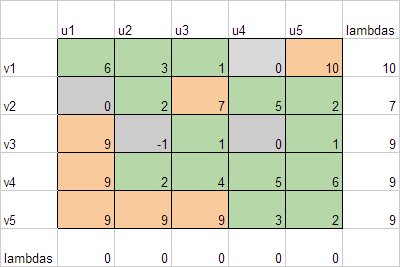
\includegraphics[width=10cm]{Homework2/OptimalAssignment1.png}    
    \end{center}\pn
    
    In the firs step, we assign the values of the dual variable \textit{lambda} 
    to be the maximum number of each row for the ``row vertices'' and zero
    for the ``column vertices''. (The name ``dual variable'' is given
    because of \href{http://www.mpi-inf.mpg.de/departments/d1/teaching/ss12/AdvancedGraphAlgorithms/Slides06.pdf}{these slides}).\pn
    
    Then we color red an ``as good as possible'' matching. This can be not necessarily perfect.
    The algorithm is going to lead us to a perfect matching with maximum weight.\pn 
    
    \begin{center}
        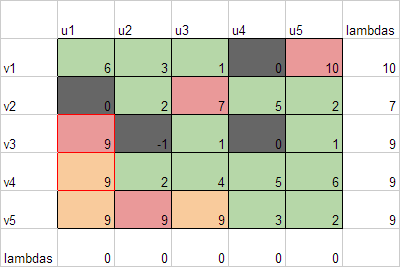
\includegraphics[width=10cm]{Homework2/OptimalAssignment2.png}        
    \end{center}\pn
    
    In the next steps we are going to try to construct an aumenting path on
    an alternat tree rooted in a not covered vertex ($v_4$ in this example) by using
    the Hungarian algorithm. It is rooted in $v_4$ because this vertex is not covered by the
    matching. We could have chosen $u_4$ instead of $v_4$.\pn
    
    Edges such that its weight is equal to the sum of the dual variable evaluated in 
    its adjacent vertices are called \textbf{thight edges}. Orange cells are thight edges
    that do not belong to the matching.
    
    Cells with red border represent the edges in the tree.\pn
    
    In the next step, we try to find an augmenting path. If we do, we augment our
    tree with such path. And we repeat this until there is not augmenting path. In
    this case, there is not such path, so we proceed to the next step.
    
    In the next step, we modify the dual variable \textit{lambda} by substracting
    $3$ to its values on ``row vertices'' that belong to the tree and by adding
    $3$ to its values on ``column vertices'' that belong to the tree.\pn
    
    $3$ is the minimum weight needed to add new orange cells that could extend
    our tree.\pn
   
    \begin{center}
        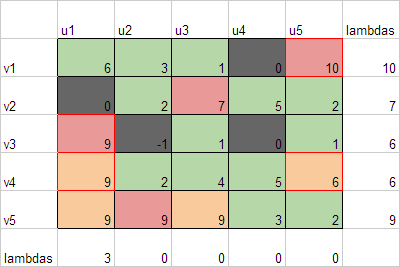
\includegraphics[width=10cm]{Homework2/OptimalAssignment3.png}
    \end{center}\pn

    After the addition of the new orange cells we extend the tree looking for an
    augmenting path. If we can't find one, then we repeat the steps from the one
    in which we modify the dual variable \textit{lambda}. 
    
    The next picture shows this repeating steps but now by substracting and adding $1$
    respectively.

    \begin{center}
        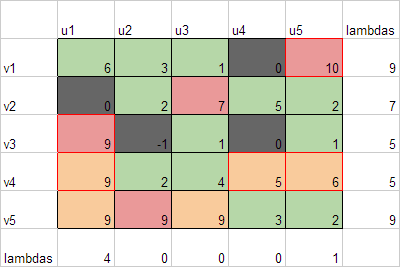
\includegraphics[width=10cm]{Homework2/OptimalAssignment4.png}
    \end{center}\pn

    Finally, the only edge added in this last step starts and ends in uncovered
    vertices. So this edge by itself is an augmenting path wich can complete
    an optimal assignment by being added to the matching.\pn
    
    In the next picture we show the optimal matching.\pn

    \begin{center}
        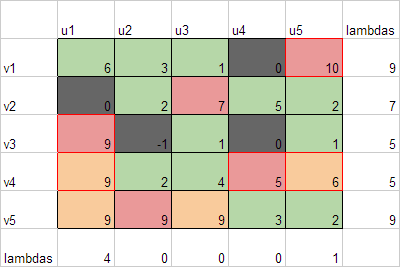
\includegraphics[width=10cm]{Homework2/OptimalAssignment5.png}
    \end{center}
    
    We can tell that this matching is optimal because the sum of all the
    values of the dual variable \textit{lambda} is $40$ and it coincides with
    the sum of the weights of the edges in the matching.
\end{proof}